\documentclass[a4paper,runningheads]{llncs}

\usepackage[T1]{fontenc}
\usepackage{graphicx}
\usepackage{amsmath}
\usepackage{url}
\usepackage{placeins}
\emergencystretch=3em

\begin{document}

\title{Controlled Acoustic Interventions for Neutral-to-Angry Prediction Shifts in Vietnamese Speech Emotion Recognition}
\titlerunning{Controlled Acoustic Interventions in Vietnamese SER}

\author{Anonymous Authors}
\authorrunning{Anonymous Authors}
\institute{Anonymous submission}

\maketitle

\begin{abstract}
Speech emotion recognition (SER) systems can change their predictions when selected acoustic properties are modified, but the cue-specific responses of Vietnamese SER systems have received limited controlled analysis. We study how pitch, energy, duration, and their combinations shift predictions from Neutral toward Angry in ViSEC. Four systems were evaluated under one frozen four-class protocol: Mel-CNN, RawWave-CNN, Wav2Vec2, and Prosody-Fusion. RQ1 used model-specific baseline-correct Neutral subsets and showed that pitch produced the most consistent Angry-directed response across the three compact systems, although RawWave-CNN was numerically more responsive to Duration than Pitch. Sham, reverse-direction, dose, and F0-component controls linked the pitch response primarily to F0-baseline elevation rather than F0-range expansion. RQ2 used the same waveforms on a strict four-model common subset ($N=36$) and found different intervention-sensitivity profiles for Pitch, Energy, and Duration; a paired analysis on all 227 true-Neutral utterances preserved this cross-pipeline heterogeneity. Supporting audits showed that preprocessing strongly changes the observability of the Energy intervention and that removing explicit F0 features substantially reduces, but does not eliminate, Prosody-Fusion pitch sensitivity. RQ3 was exploratory: the pooled F0-baseline response was positive in the North, Central, and South metadata groups, but architecture-specific responses were heterogeneous and speaker coverage was limited. Objective checks confirmed the intended F0 shift, high local-contour correlation, zero duration drift, small mean RMS drift, and no clipping. The results characterize model-level sensitivity under a fixed diagnostic protocol; they do not establish perceptual anger, natural emotional conversion, lexical-tone preservation, or universal cue importance.

\keywords{Vietnamese speech emotion recognition \and Acoustic intervention \and Fundamental frequency \and Model sensitivity \and Accent metadata}
\end{abstract}

\section{Introduction}

Speech emotion recognition maps speech to discrete or continuous affective predictions. Performance summaries alone do not show which acoustic changes move a trained system between classes, and systems with similar accuracy may respond differently to the same waveform intervention. Controlled interventions provide a model-level diagnostic: one can modify a selected acoustic dimension, hold the input identity fixed, and measure the resulting change in class probability. This does not imply that the modified utterance is natural or that a listener perceives the intended emotion.

Vietnamese makes this distinction especially important. Fundamental frequency (F0) carries both prosodic and lexical-tone information, while emotion-related variation can involve F0, energy, timing, voice quality, and their interactions. Vietnamese SER work has emphasized pitch-aware modeling and tonal-language considerations \cite{thanh2024pitchfusion,ngo2012vietnameseprosody}, but matched interventions across different model families remain underexplored. General SER reviews likewise identify preprocessing, representations, and evaluation design as major sources of variation \cite{akcay2020ser,madanian2023ser}.

We investigate one locked model-level objective: how controlled acoustic changes cause SER systems to shift their predictions from Neutral toward Angry in Vietnamese speech. The scientific narrative proceeds from acoustic cues, to comparative model sensitivity, to exploratory accent variation. We ask:

\begin{enumerate}
    \item \textbf{RQ1 -- Acoustic Cue Sensitivity:} Which tested acoustic components most strongly shift Neutral predictions toward Angry in Vietnamese speech emotion recognition?
    \item \textbf{RQ2 -- Architecture-Dependent Sensitivity:} Do different SER model families exhibit distinct sensitivity profiles under the same acoustic interventions?
    \item \textbf{RQ3 -- Accent-Dependent F0 Sensitivity:} How does F0-baseline sensitivity vary across the North, Central, and South Vietnamese accent groups represented in ViSEC?
\end{enumerate}

The term ``architecture-dependent'' in RQ2 denotes an empirical comparison between complete systems. Observed differences may arise from architecture, preprocessing, feature access, and training; the experiment does not isolate architecture as a causal factor. The novelty is therefore not a new classifier, but a controlled, within-utterance diagnostic that connects cue-specific probability shifts, discrete Neutral-to-Angry flips, matched cross-pipeline comparisons, and intervention-validity controls in Vietnamese SER. The contributions are: (i) a controlled comparison of pitch, energy, duration, and cue combinations; (ii) matched four-system sensitivity analysis with sham, direction, dose, and robustness controls; and (iii) an exploratory accent-stratified analysis with explicit speaker and metadata limitations. Preprocessing observability and an explicit-F0 ablation are supporting analyses for RQ2, not new research questions.

\section{Related Work}

SER systems use spectral, waveform, self-supervised, and prosodic representations, with results affected by corpus composition, speaker partitioning, preprocessing, and evaluation protocol \cite{akcay2020ser,madanian2023ser}. Wav2vec~2.0 provides self-supervised speech representations that can be fine-tuned for downstream classification \cite{baevski2020wav2vec2}. Pitch-Fusion was proposed for emotion recognition in tonal languages and introduced the ViSEC setting used here \cite{thanh2024pitchfusion}; earlier Vietnamese work also documented emotion-related changes in F0, power, and duration \cite{ngo2012vietnameseprosody}.

Vocal emotion is conveyed by coordinated acoustic profiles rather than a single universally sufficient cue \cite{scherer1991vocal}. This motivates interventions that separately alter F0 baseline, F0 range, energy, and duration, followed by combination tests. Our transformations are diagnostic perturbations rather than emotional voice conversion: they are not optimized for naturalness, speaker identity, or perceived emotion.

Pitch-synchronous overlap-add methods provide a standard basis for waveform-level pitch manipulation \cite{moulines1990psola}. We use the Parselmouth interface \cite{jadoul2018parselmouth} to apply PSOLA and include zero-shift resynthesis, reverse-direction, and dose controls. The research gap is therefore narrow: under one Vietnamese dataset split, do matched acoustic interventions produce systematic and different Neutral-to-Angry probability shifts across complete SER systems, and how do those responses vary across the accent metadata represented in the corpus?

\section{Methodology}

\subsection{Dataset and Frozen Protocol}

We used ViSEC only. The staged corpus contained 5,280 utterances with four labels: Happy, Neutral, Sad, and Angry, mapped to 0, 1, 2, and 3. Because no valid predefined split was available, a weighted 70/15/15 split was generated with seed 2025 and then frozen: 3,611 training, 828 validation, and 841 test utterances. Table~\ref{tab:split} reports the label counts. Audio was sampled at 16~kHz and cropped or padded to 4.5~s.

\begin{table}[!htbp]
\caption{Emotion counts in the frozen ViSEC split.}
\label{tab:split}
\centering
\begin{tabular}{lrrrrr}
\hline
Split & Angry & Happy & Neutral & Sad & Total \\
\hline
Train & 998 & 806 & 1,044 & 763 & 3,611 \\
Validation & 217 & 212 & 236 & 163 & 828 \\
Test & 251 & 210 & 227 & 153 & 841 \\
\hline
\end{tabular}
\end{table}

Identified speaker IDs were disjoint across splits (128 training, 9 validation, and 12 test IDs). Speaker ID 0 is a heterogeneous missing-ID bucket containing 2,217 files; those files were stratified by emotion and accent, so complete speaker independence cannot be guaranteed for that bucket. Exact full-WAV and decoded-PCM hashes found no cross-split duplicates. The local corpus came from a Parquet-derived ViSEC mirror whose official distribution version or commit could not be established.

\subsection{SER Systems}

We evaluated four complete SER systems. Mel-CNN used two-dimensional convolution over per-utterance normalized log-Mel input. RawWave-CNN used one-dimensional convolution over the fixed-length waveform without amplitude normalization after loading. Wav2Vec2 used the pretrained \texttt{nguyenvulebinh/}\allowbreak\texttt{wav2vec2-base-}\allowbreak\texttt{vietnamese-250h} checkpoint, whose feature extractor performs input normalization, and was fine-tuned on the same split. Prosody-Fusion combined a Mel CNN with standardized explicit log-F0 mean, log-F0 standard deviation, log-RMS, and duration features.

For each system, final predictions were the arithmetic mean of class-probability vectors from seeds 2025, 2026, and 2027. Compact-model learning rates were selected by validation Macro-F1: $3\times10^{-4}$ for Mel-CNN and RawWave-CNN, and $8\times10^{-4}$ for Prosody-Fusion. Wav2Vec2 used class-weighted cross-entropy, a frozen convolutional feature encoder, mixed precision, and effective batch size 16; validation-only comparison selected $3\times10^{-5}$. Temperature scaling for robustness analysis was fitted on validation predictions only, following the calibration setting of Guo et al. \cite{guo2017calibration}.

\subsection{Controlled Acoustic Interventions}

All transformation parameters were estimated from training-set Neutral and Angry utterances. The pooled means were 5.232584 and 5.580303 log-Hz, producing a Neutral-to-Angry shift of 0.347719 log-Hz and an F0 ratio of 1.415834. Neutral and Angry log-F0 standard deviations were 0.257408 and 0.246862. The train-derived Angry-minus-Neutral log-RMS shift was $-0.203997$, and the duration factor was 0.807767.

Pitch was transformed with Parselmouth PSOLA using a 10-ms analysis step and a 60--500~Hz search range. The full pitch mapping was
\begin{equation}
\log F'_{0,t}=\mu_A+\frac{\sigma_A}{\sigma_N}\left(\log F_{0,t}-\mu_N\right),
\end{equation}
where $A$ and $N$ denote Angry and Neutral training statistics. The mean-only condition used
\begin{equation}
\log F'_{0,t}=\log F_{0,t}+(\mu_A-\mu_N).
\end{equation}
The range-only condition modified contour range without the baseline shift; Reverse F0 used the opposite-direction shift. Zero-shift PSOLA resynthesis served as the sham. Pitch and duration outputs were restored to the input mean log-RMS. Combination order was Pitch, Duration, then Energy, with peak protection only when needed.

The intervention set comprised Pitch, Energy, Duration, Pitch + Energy, Pitch + Duration, Energy + Duration, and all three components. The original dose grid applied 25\%, 50\%, 75\%, and 100\% of the train-pooled shift, with 125\% as a stress condition. A later fixed-dose audit used $-2$, 0, +1, +2, +3, +4, and +6 semitones on all 227 Neutral test utterances. These are different protocols: the pooled training contrast was 6.020 semitones, whereas the within-speaker contrast among 58 identified speakers represented in both emotions was 3.977 semitones. We therefore interpret +4 semitones as the primary fixed-dose check and +6 semitones as a stress test.

\subsection{Analysis Populations and Outcomes}

For utterance $i$, the principal continuous outcome was
\begin{equation}
\Delta P_i(\mathrm{Angry})=P_i(\mathrm{Angry}\mid\mathrm{transformed})-P_i(\mathrm{Angry}\mid\mathrm{baseline}).
\end{equation}
Angry Flip Rate was the fraction of baseline-Neutral predictions whose transformed argmax became Angry. Thus $Delta P(\mathrm{Angry})$ measures a continuous change in model confidence even when the predicted class is unchanged, whereas Angry Flip Rate records only a discrete Neutral-to-Angry decision change. The two quantities are complementary and are not interchangeable.

RQ1 used model-specific subsets of true Neutral test utterances correctly predicted as Neutral at baseline: $N=140$ for Mel-CNN, $N=90$ for RawWave-CNN, and $N=136$ for Prosody-Fusion. Its full sham, direction, dose, and F0-component control suite was executed for these three compact systems. Wav2Vec2 was added as the strong self-supervised comparison for RQ2; because matching outputs for the original RQ1 control suite were not available, we did not retrofit it into RQ1 with a non-equivalent protocol. Wav2Vec2 is nevertheless included in the four-system fixed-dose audit and every RQ2 comparison. RQ2 used the strict intersection correctly classified as Neutral by all four systems ($N=36$); waveform SHA-256 hashes verified that each system received the same transformed waveform. A secondary paired RQ2 robustness analysis used all 227 true Neutral utterances without conditioning on baseline correctness. That broader analysis estimates probability sensitivity only; its population is not valid for a common Angry Flip Rate denominator. The fixed-dose audit and RQ3 also used all 227 true Neutral test utterances with valid accent metadata. In RQ3, the baseline was the original waveform and the intervention was the original 100\% train-derived F0-mean condition.

RQ1 used paired Wilcoxon signed-rank tests with Holm correction and matched rank-biserial effect sizes. Mean $\Delta P(\mathrm{Angry})$ confidence intervals were obtained by bootstrap. RQ2 used separate Friedman tests for Pitch, Energy, and Duration, with Kendall's $W$ and Holm-corrected paired Wilcoxon follow-ups. The same paired tests were repeated as a secondary robustness analysis on all 227 true Neutral utterances. RQ3 used a repeated-utterance generalized estimating equation with utterance as the cluster and accent, system, and their interaction as predictors \cite{liang1986gee}; architecture-specific Kruskal-Wallis and Holm-corrected Mann-Whitney analyses were supporting checks. The significance threshold was $\alpha=0.05$.

\section{Results}

\subsection{Baseline SER Performance}

Table~\ref{tab:baseline} reports test Macro-F1 across seeds. Wav2Vec2 was the strongest baseline classifier, but classification performance did not determine intervention sensitivity. Its three-member probability ensemble achieved Macro-F1 0.6792 and accuracy 0.6873; class F1 values were 0.6005 (Happy), 0.6285 (Neutral), 0.6733 (Sad), and 0.8147 (Angry).

\begin{table}[!htbp]
\caption{Test Macro-F1 across three independent seeds.}
\label{tab:baseline}
\centering
\begin{tabular}{lrr}
\hline
System & Mean & SD \\
\hline
Mel-CNN & 0.4451 & 0.0192 \\
RawWave-CNN & 0.4366 & 0.0091 \\
Wav2Vec2 & 0.6513 & 0.0214 \\
Prosody-Fusion & 0.4702 & 0.0074 \\
\hline
\end{tabular}
\end{table}

\subsection{RQ1: Acoustic Cue Contributions}

Figure~\ref{fig:rq1} summarizes the single-component effects on the model-specific baseline-correct subsets. Pitch increased Angry probability in all three systems. Energy did not show a consistent positive response. Duration was positive for RawWave-CNN (0.0315) but negative for Mel-CNN ($-0.0272$) and Prosody-Fusion ($-0.0121$). For Mel-CNN, Angry Flip Rates for Pitch, Energy, and Duration were 2.14\%, 2.14\%, and 0\%; for RawWave-CNN they were 1.11\%, 0\%, and 7.78\%; and for Prosody-Fusion they were 17.65\%, 0\%, and 0\%. These discrete rates are reported alongside, rather than substituted for, the continuous probability effects.

\begin{figure}[!htbp]
\centering
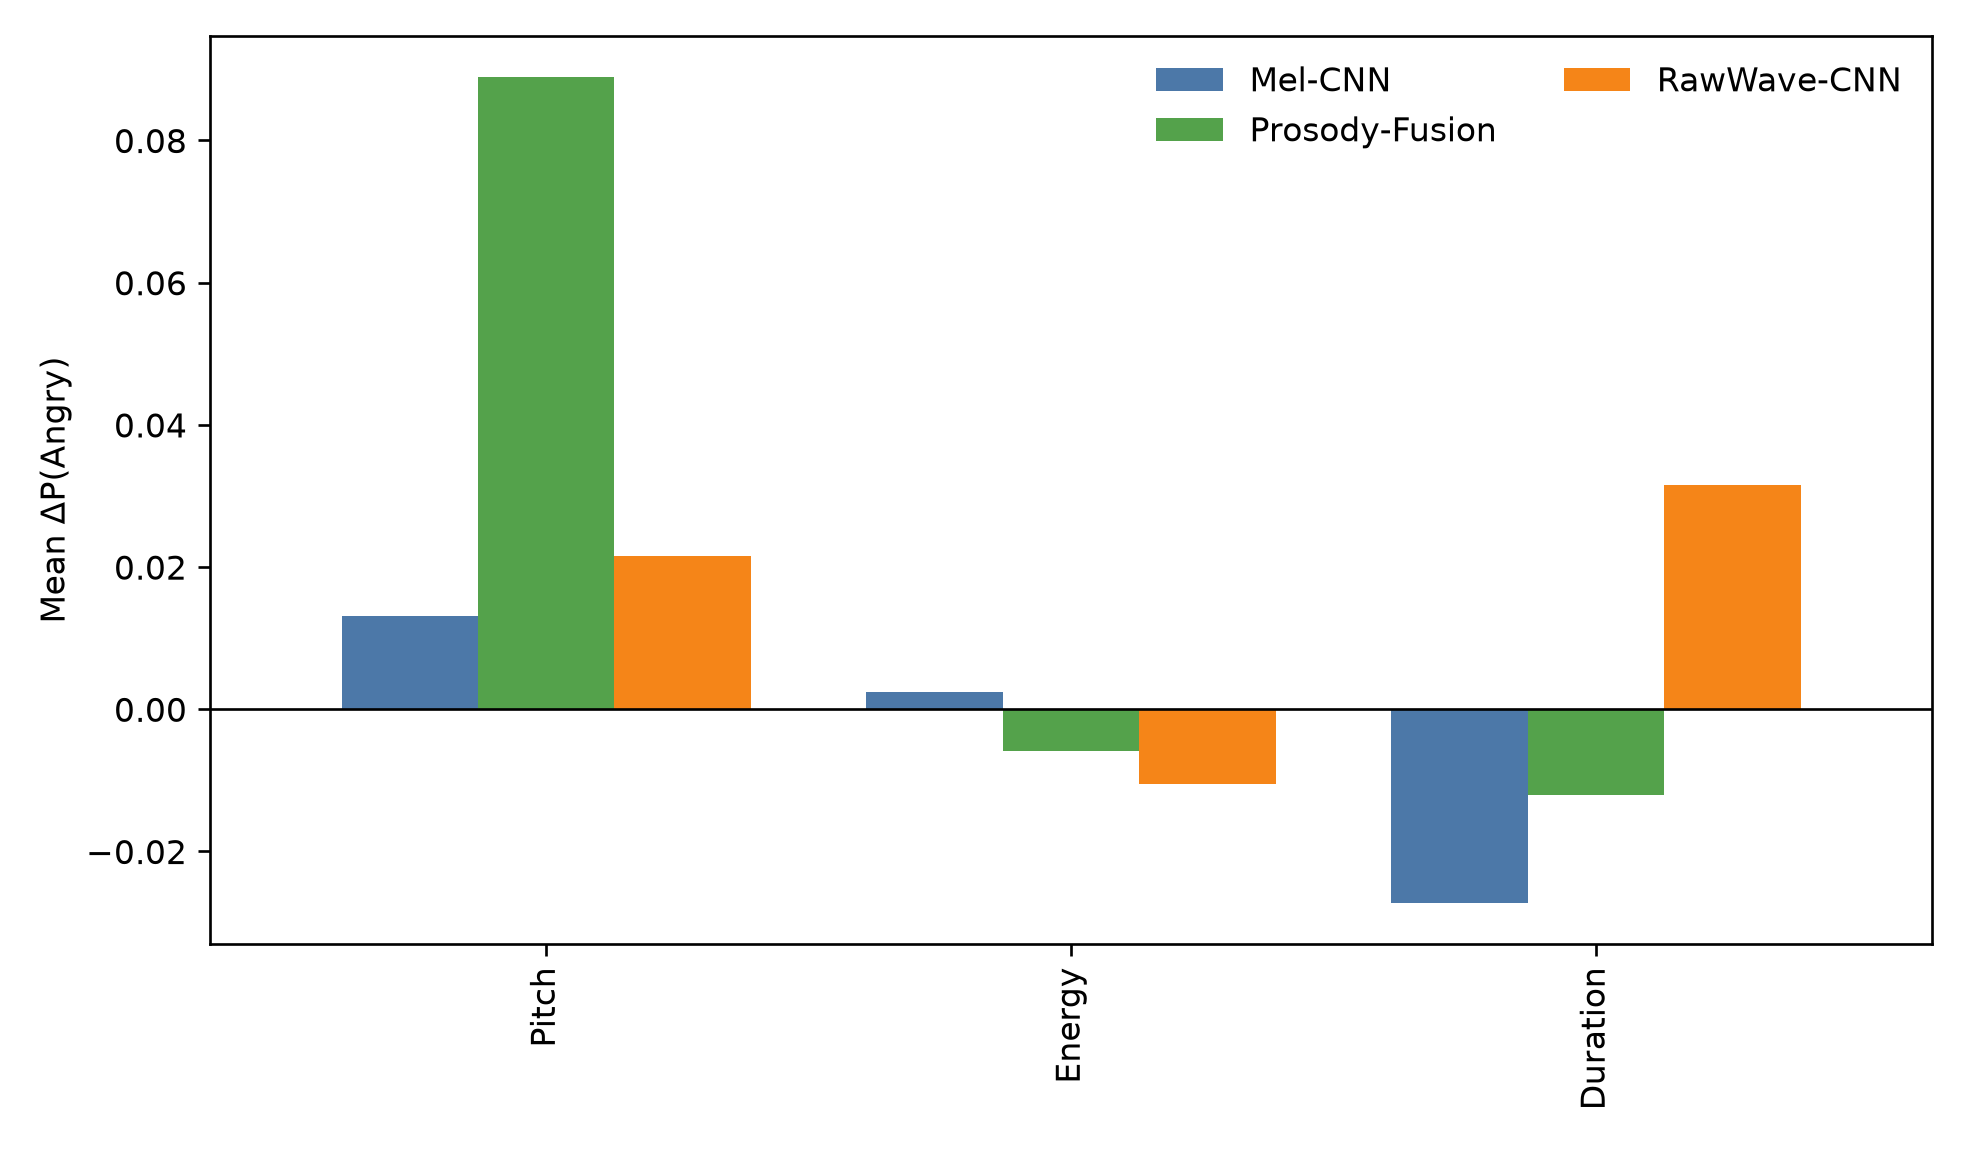
\includegraphics[width=\textwidth]{figures/rq1_single_components.png}
\caption{RQ1 single-component mean $\Delta P(\mathrm{Angry})$. Each system uses its own baseline-correct Neutral subset; the bars must not be interpreted as one shared sample.}
\label{fig:rq1}
\end{figure}

Pitch exceeded Energy after Holm correction in all three systems: mean paired differences were 0.0107 (Mel-CNN, adjusted $p=6.08\times10^{-10}$, rank-biserial $r=0.603$), 0.0321 (RawWave-CNN, $p=4.70\times10^{-13}$, $r=0.896$), and 0.0947 (Prosody-Fusion, $p=1.47\times10^{-23}$, $r=0.999$). Pitch also exceeded Duration for Mel-CNN and Prosody-Fusion. RawWave-CNN was the exception: Pitch minus Duration was $-0.0099$ and not significant after correction ($p=0.0840$).

The control analyses support an F0-baseline interpretation within this protocol. The 100\% Pitch condition exceeded PSOLA sham in all three systems, with mean paired differences of 0.0229, 0.0220, and 0.0896. Angry-directed Pitch exceeded Reverse Pitch in each system. F0 mean-only also exceeded F0 range-only, with differences of 0.0288 (Mel-CNN), 0.0237 (RawWave-CNN), and 0.0971 (Prosody-Fusion), all significant after correction. The architecture-mean sham-relative effect increased from 0.0059 at 25\% to 0.0448 at 100\% and 0.0561 at the 125\% stress condition, although RawWave-CNN's 25\% and 50\% effects did not survive Holm correction.

The fixed-dose audit on all 227 Neutral utterances qualified the large pooled shift. At +4 semitones, mean $\Delta P(\mathrm{Angry})$ was 0.0044 [0.0016, 0.0071] for Mel-CNN, 0.0207 [0.0163, 0.0252] for RawWave-CNN, $-0.0038$ [$-0.0185$, 0.0101] for Wav2Vec2, and 0.0579 [0.0507, 0.0649] for Prosody-Fusion. Thus Wav2Vec2 was not clearly positive at +4 semitones. At the +6-semitone stress dose, the corresponding means were 0.0141, 0.0402, 0.0130, and 0.0890. Overall, F0-baseline manipulation produced the most consistent Angry-directed response among the tested cues, but it was not universally dominant: RawWave-CNN retained a distinct Duration-sensitive pattern, and Wav2Vec2's +4-semitone interval included zero.

\subsection{RQ2: Cross-Model Sensitivity}

The strict common subset contained 36 true Neutral utterances correctly classified as Neutral by all four systems. Table~\ref{tab:rq2} and Fig.~\ref{fig:rq2} show that the response ordering depended on the intervention. Prosody-Fusion was most responsive to Pitch, whereas RawWave-CNN was most responsive to Pitch+Duration and showed a positive Duration response. Mel-CNN and Wav2Vec2 had smaller Pitch responses on this subset.

\begin{table}[!htbp]
\caption{Mean $\Delta P(\mathrm{Angry})$ on the shared RQ2 subset ($N=36$).}
\label{tab:rq2}
\centering
\resizebox{\textwidth}{!}{%
\begin{tabular}{lrrrrrrr}
\hline
System & Pitch & Energy & Duration & P+E & P+D & E+D & All \\
\hline
Mel-CNN & 0.0066 & 0.0003 & $-0.0093$ & 0.0072 & $-0.0088$ & $-0.0089$ & $-0.0084$ \\
RawWave-CNN & 0.0302 & $-0.0115$ & 0.0310 & 0.0188 & 0.0523 & 0.0232 & 0.0449 \\
Wav2Vec2 & 0.0099 & $\approx0$ & $-0.0159$ & 0.0099 & $-0.0003$ & $-0.0159$ & $-0.0003$ \\
Prosody-Fusion & 0.0536 & $-0.0056$ & $-0.0065$ & 0.0491 & 0.0396 & $-0.0114$ & 0.0353 \\
\hline
\end{tabular}}
\end{table}

\begin{figure}[!htbp]
\centering
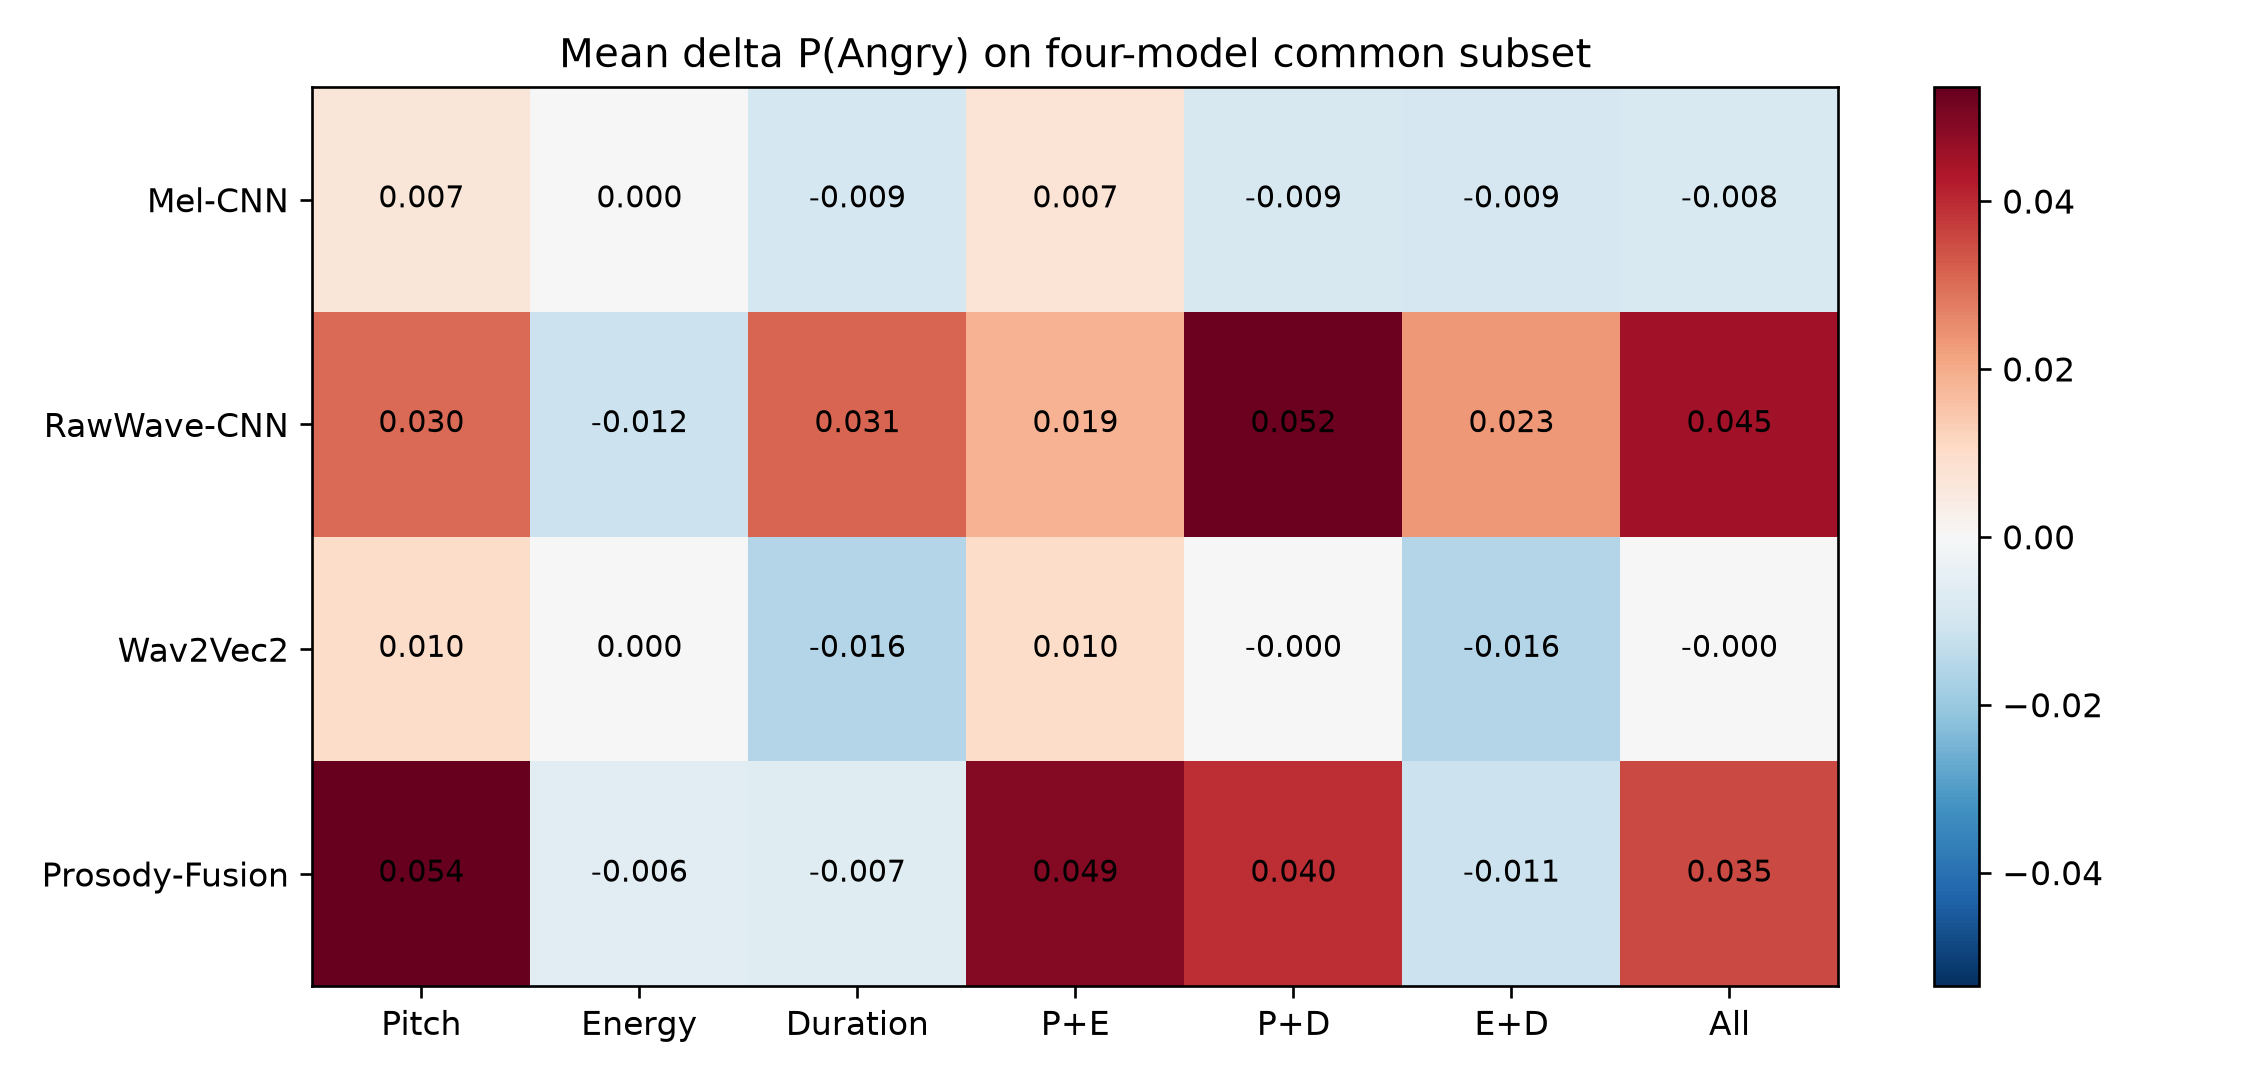
\includegraphics[width=\textwidth]{figures/rq2_intervention_heatmap.png}
\caption{Four-system intervention-sensitivity profiles on the shared $N=36$ subset. Values are probability differences, not classification accuracy.}
\label{fig:rq2}
\end{figure}

\FloatBarrier
The Friedman tests were significant for Pitch ($\chi^2=57.200$, $p=2.33\times10^{-12}$, $W=0.530$), Energy ($\chi^2=49.733$, $p=9.11\times10^{-11}$, $W=0.460$), and Duration ($\chi^2=43.633$, $p=1.81\times10^{-9}$, $W=0.404$). For Pitch, five of six paired comparisons survived Holm correction; Mel-CNN versus Wav2Vec2 did not ($p=0.0854$). Pairwise Spearman correlations between the seven-intervention rankings ranged from $-0.464$ to 0.929. Only Mel-CNN versus Wav2Vec2 survived Holm correction ($\rho=0.929$, adjusted $p=0.0151$), and this ranking analysis is supporting evidence because only seven conditions were ranked.

The paired all-Neutral analysis strengthened the sample-size robustness check without changing the estimand of the primary baseline-correct analysis. On the same 227 utterances for all four pipelines, mean Pitch responses were 0.0109 (Mel-CNN), 0.0386 (RawWave-CNN), 0.0100 (Wav2Vec2), and 0.0860 (Prosody-Fusion); Energy responses were 0.0034, $-0.0076$, approximately 0, and $-0.0057$; and Duration responses were $-0.0378$, 0.0278, $-0.0524$, and $-0.0202$. Friedman tests remained significant for Pitch ($\chi^2=311.733$, $p=2.87\times10^{-67}$, $W=0.458$), Energy ($\chi^2=291.122$, $p=8.30\times10^{-63}$, $W=0.427$), and Duration ($\chi^2=240.938$, $p=5.96\times10^{-52}$, $W=0.354$). All six Pitch pairs survived Holm correction; the only nonsignificant pairs were RawWave-CNN versus Prosody-Fusion for Energy ($p=0.315$) and Mel-CNN versus Wav2Vec2 for Duration ($p=0.348$). Validation-only temperature scaling and this broader paired analysis therefore preserved the principal qualitative heterogeneity. Because baseline predictions differ across systems in this set, these results support probability-sensitivity differences, not a four-system flip-rate comparison.

Two supporting audits clarify, rather than replace, the RQ2 result. First, the Energy intervention changed the waveform by 0.184535 relative L2 and $-1.772$~dB. After preprocessing, mean relative L2 was 0.017410 for normalized log-Mel and 0.000079 for Wav2Vec2, while RawWave-CNN retained 0.184535; Prosody-Fusion additionally received a standardized log-RMS displacement of 0.185808. Near-zero Wav2Vec2 Energy response is therefore a property of its complete pipeline and must not be read as proof that its learned representation ignores energy.

Second, removing explicit F0 mean and F0 standard deviation from Prosody-Fusion reduced mean baseline Macro-F1 from 0.4702 to 0.4422. At +4 semitones, mean $\Delta P(\mathrm{Angry})$ fell from 0.0579 to 0.0118. The paired sham-adjusted full-minus-no-F0 difference was 0.0351 [0.0297, 0.0407], Wilcoxon $p=2.09\times10^{-30}$, rank-biserial $r=0.877$. The no-F0 system remained pitch-sensitive through its log-Mel branch, while explicit F0 access amplified that response.

\subsection{RQ3: Exploratory Accent Analysis}

RQ3 used the original 100\% train-derived F0-mean intervention and the original waveform baseline on all 227 eligible Neutral utterances: 31 North, 25 Central, and 171 South. The pooled response first averaged the four system responses within each utterance. Mean pooled $\Delta P(\mathrm{Angry})$ was 0.0286 [0.0140, 0.0455] for North, 0.0160 [0.0028, 0.0283] for Central, and 0.0455 [0.0374, 0.0536] for South.

\begin{figure}[!htbp]
\centering
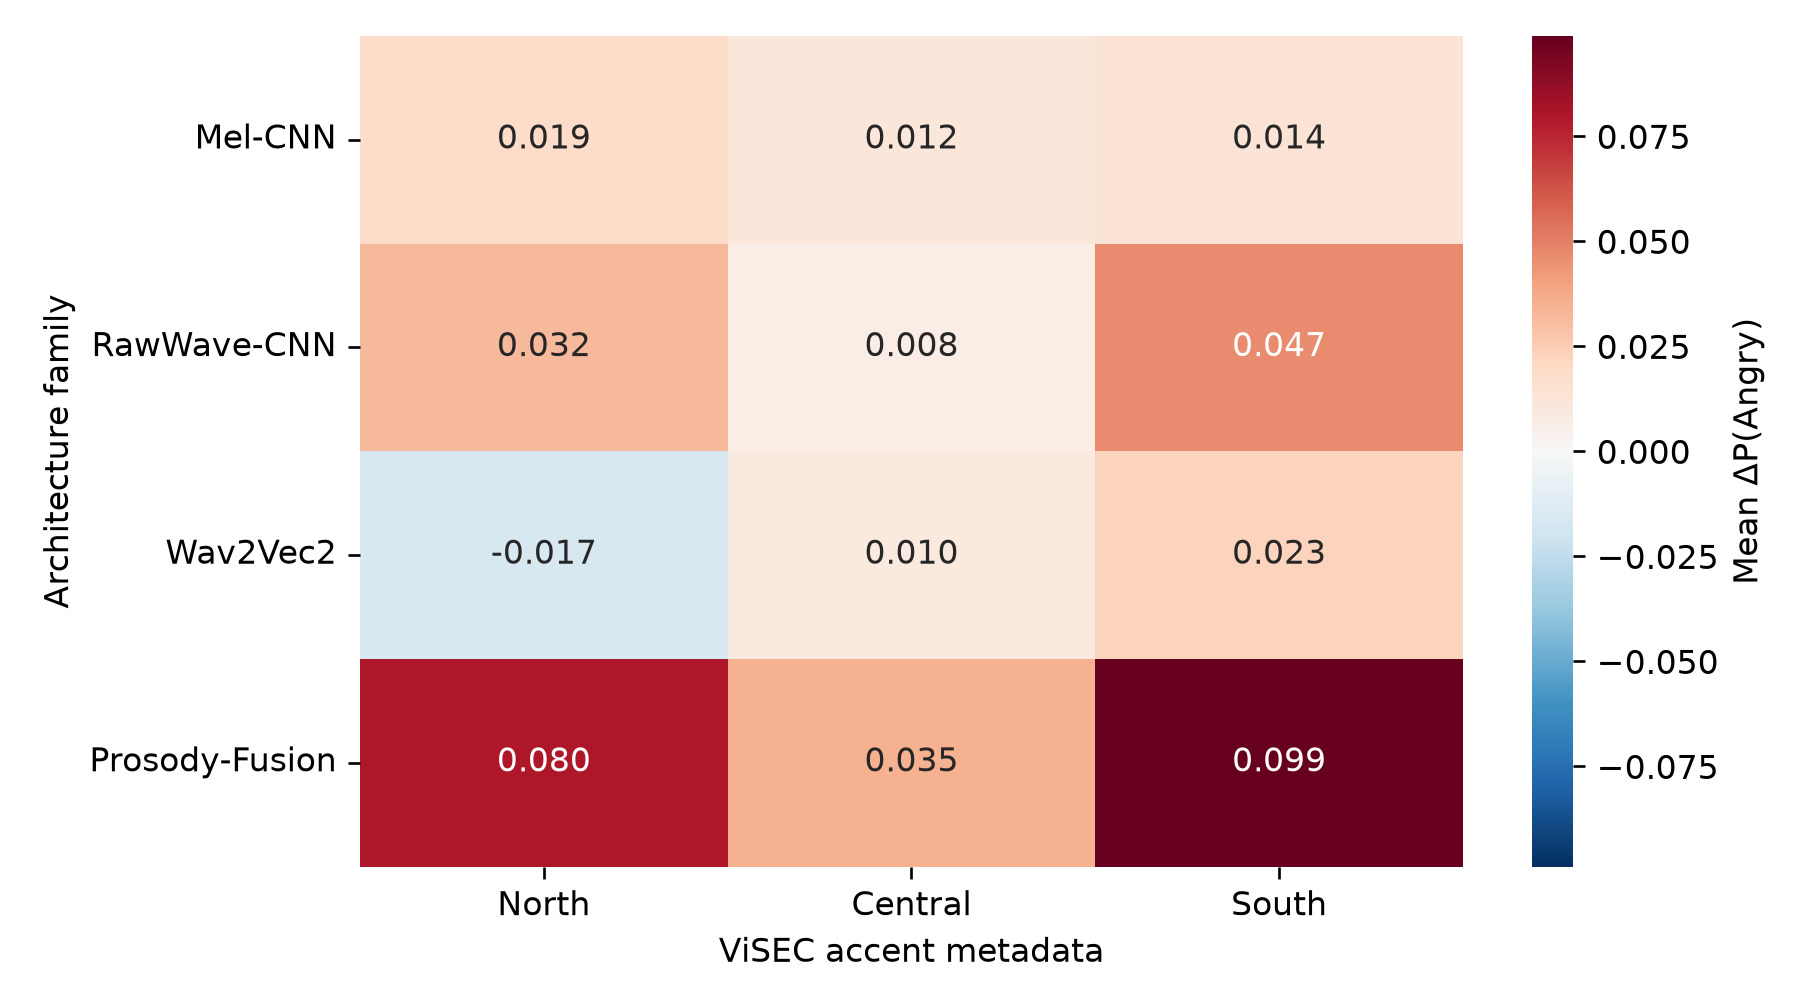
\includegraphics[width=0.88\textwidth]{figures/rq3_accent_heatmap.png}
\caption{Architecture-specific mean F0-baseline response by ViSEC accent metadata. The analysis is exploratory and cannot separate accent from speaker effects.}
\label{fig:rq3}
\end{figure}

The pooled positive direction did not hold in every architecture-by-accent cell: Wav2Vec2/North was negative at $-0.0166$. In the repeated-utterance GEE, the accent joint term at the Mel-CNN reference was not significant ($p=0.2369$), whereas architecture ($p=4.74\times10^{-54}$) and architecture-by-accent interaction ($p=2.986\times10^{-14}$) were significant. Architecture-specific Kruskal-Wallis tests were significant for RawWave-CNN ($p=0.000117$, $\epsilon^2=0.0719$) and Prosody-Fusion ($p=8.38\times10^{-5}$, $\epsilon^2=0.0749$), but not for Mel-CNN or Wav2Vec2. These results show heterogeneous sensitivity in the represented metadata groups; they do not establish population-level accent differences or equivalence where tests were non-significant.

\subsection{Intervention Validity and Robustness}

Objective checks evaluated the unchanged 100\% F0-mean intervention on 227 Neutral utterances. The intended mean log-F0 shift was 0.347719 and the achieved mean shift was 0.312897; the median achieved F0 ratio was 1.414682. Median local log-F0 contour correlation was 0.990946. Maximum absolute duration drift was 0~s, mean RMS drift was $-0.036737$~dB, maximum clipping fraction was 0\%, and all transformed arrays were finite. Sham, reverse-direction, and dose-response results further show that the probability shifts were not identical to zero-shift resynthesis and generally followed intervention direction and strength.

These checks establish signal-level execution, not perceptual validity. No valid multi-rater quality-control responses were available. No Vietnamese ASR content-preservation analysis was run because aligned transcripts and a validated local ASR workflow were not available. We therefore report neither character error rate nor lexical-tone preservation.

\section{Discussion}

\paragraph{RQ1.} F0 manipulation produced the most consistent Neutral-to-Angry probability shift across the tested single components. Mean-only versus range-only, reverse-direction, sham, and dose controls associate the effect mainly with F0-baseline elevation in this protocol. The conclusion is conditional: RawWave-CNN was numerically more Duration-sensitive, Wav2Vec2 was not clearly positive at the primary +4-semitone fixed dose, and none of these model responses establishes a universal human anger cue.

\paragraph{RQ2.} The four complete systems exhibited different intervention-sensitivity profiles under matched waveforms. This conclusion held in both the strict baseline-correct subset and the broader paired $N=227$ probability analysis. Prosody-Fusion was strongly pitch-sensitive, RawWave-CNN showed a distinct Duration response, and Wav2Vec2 combined the strongest baseline Macro-F1 with comparatively modest Pitch sensitivity. The preprocessing audit demonstrates that cross-system Energy comparisons partly reflect whether the intervention reaches the model input. The no-F0 ablation gives a more specific mechanism result: explicit F0 access amplifies Prosody-Fusion sensitivity, while the remaining spectral branch retains a smaller response. Architecture, preprocessing, feature access, and training remain confounded, so an architecture-only causal claim is not supported.

\paragraph{RQ3.} The pooled F0-baseline response was positive in all three accent metadata groups, but its size and architecture-specific direction were not uniform. Central had only 25 eligible utterances, South dominated the sample, known-speaker counts were small, and 77 South utterances had missing speaker IDs. The interaction is therefore exploratory evidence of heterogeneous model response in this dataset, not a statement about how regional speakers express anger.

The combined findings support controlled interventions as a diagnostic for SER robustness. They do not demonstrate natural emotional conversion, human-perceived anger, or preservation of Vietnamese lexical tone. A future perception and content-preservation study would address those questions, but it is outside the present model-level objective.

\section{Limitations}

The locally generated split was necessary because a valid predefined split was unavailable, and the official commit of the Parquet-derived ViSEC mirror is unknown. Identified speakers were disjoint, but the heterogeneous missing-ID bucket prevents a complete speaker-independence guarantee. RQ1 uses different baseline-correct subsets for each compact model, while RQ2's strict common subset is small ($N=36$). The fixed-dose all-Neutral audit answers a different question and must not be conflated with baseline-correct flip-rate analysis. Cross-system comparisons do not isolate architecture from preprocessing, feature access, and training. Accent groups are imbalanced and confounded with sparse speaker coverage. PSOLA and time-scale modification may introduce audible artifacts even when objective checks pass. No valid multi-rater perception evidence, character-error analysis, or lexical-tone preservation result is available. Finally, test metrics were materialized for candidate training runs; no code path used them for selection, but analyst blinding cannot be independently verified.

\section{Conclusion}

Controlled acoustic interventions revealed systematic but qualified Neutral-to-Angry prediction shifts in Vietnamese SER. For RQ1, F0-baseline elevation produced the most consistent response among the three systems with the complete control suite, with RawWave-CNN Duration sensitivity as an important exception; the separate four-system fixed-dose audit showed that Wav2Vec2 was weak at +4 semitones. For RQ2, matched waveforms produced different complete-system sensitivity profiles on both $N=36$ baseline-correct and $N=227$ all-true-Neutral paired analyses, partly shaped by preprocessing observability and explicit F0 access. For RQ3, pooled responses were positive across the represented accent groups, but architecture-specific effects were heterogeneous and the analysis remains exploratory. These conclusions apply to the evaluated checkpoints and protocol and should not be extended to human emotion perception or Vietnamese speech generally.

\paragraph{Disclosure of Interests.} The authors should complete this declaration before submission.

\bibliographystyle{splncs04}
\bibliography{references}

\end{document}
